
\documentclass[letterpaper,11pt]{article}
\usepackage[utf8]{inputenc}
\usepackage[spanish]{babel}
\usepackage{mathtools}

\begin{document}

\title{Análisis de algoritmos iterativos y recursivos\\\large Actividad 2}
\author{Dagoberto Quevedo}
\maketitle

\begin{abstract}
En esta actividad se realiza realizar una implementación recursiva e iterativa de los siguientes algoritmos: (a) Búsqueda binaria y (b) Exponenciación entera. Para cada implementación evaluar con distintas instancias su eficiencia en términos de tiempo de ejecución y se identifican las instancias que generan el peor caso.
\end{abstract}

\section{Exponenciación entera}

La exponenciación entera consiste en computar la potencia $a^b$, esto se deriva de una definición abreviada de la multiplicación siguiente $a^b=a\times a \dots^b \dots \times a$, donde $b$ es el número de veces que $a$ se multiplica a si mismo. En el caso de la exponenciación, cuando el componente $b$ de la operación es par se tiene que,
\begin{equation}
	a^b = [a \times \dots ^{b/2} \dots \times a] \times [a \times \dots ^{b/2} \dots \times a]  = a^{b/2} \times a^{b/2},
	%\dots \dots \times a \] \times \[a\times \dots  \dots \times a \]
\end{equation}
por lo cual, la definición recursiva de esta operación puede definirse como sigue,
\[
    a^b= 
\begin{cases}
    a^{b/2} \times a^{b/2}	,& \text{si } b> 0 \text{ y }  b \bmod 2 = 0, \\
    a\times a^{b-1}		,& \text{si } b> 0 \text{ y }  b \bmod 2 > 0, \\
    1					,& \text{si } b>0.
\end{cases}
\]
\subsection{Implementación y condiciones de experimentación}
Se realiza la implementación recursiva e iterativa de la operación en Python, la evaluación se realiza ejecutando una serie de instancias, en este caso cada instancia se define $a^{2^1} \dots a^{2^n}$, donde $a=1000$ y $n=25$, la ejecución se repite $k=5$ veces.

\subsection{Resultados}
El gráfico \ref{fig:ie} muestra los resultados del diseño experimental en el tiempo de computo expresado en escala logarítmica, el eje vertical expresa el valor de $n$ que define la instancia $a^{2^n}$.

\begin{figure}[h!]
  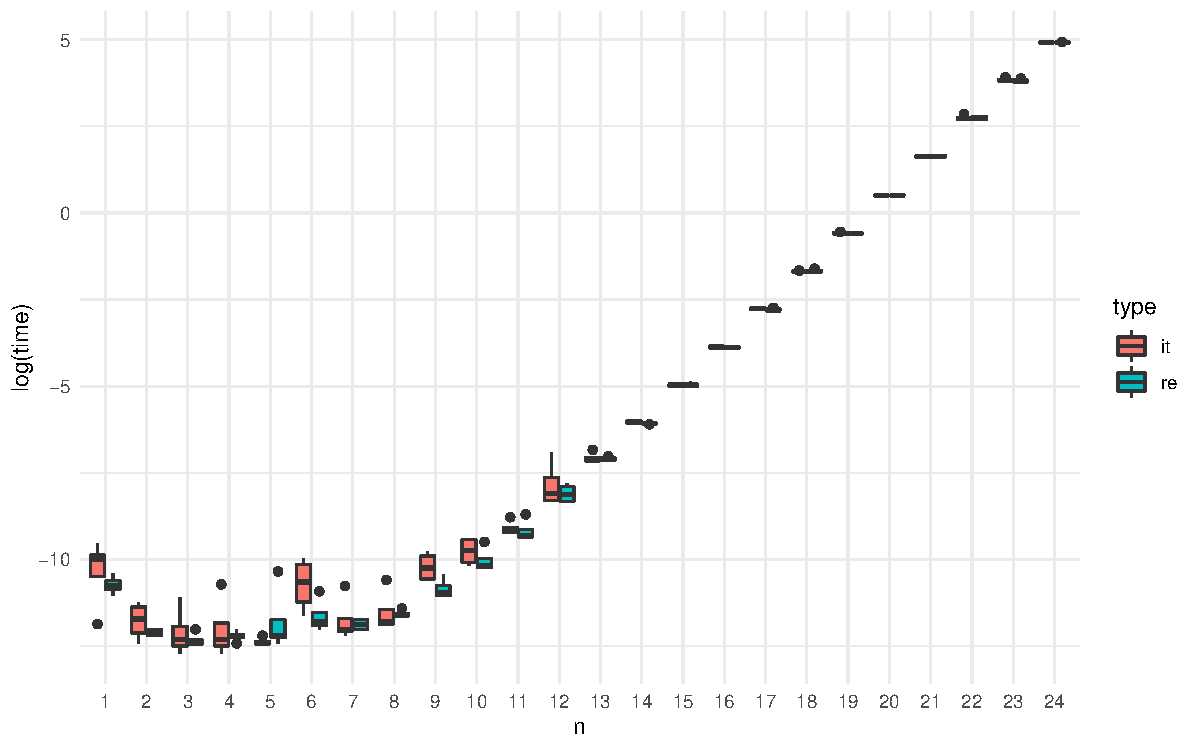
\includegraphics[width=\linewidth]{ie.pdf}
  \caption{Resultados del diseño experimental con $k=5$ ejecuciones para cada tipo de implementación e instancia de prueba}
  \label{fig:ie}
\end{figure}

Los resultados muestran que no existe evidencia suficiente a partir del tiempo de computo para concluir que una implementación es mejor que otra, esto debido a que el número de operaciones requerido para ambas implementaciones es aproximadamente igual.

\section{Búsqueda binaria}

La definición formal de la búsqueda binaria consiste en la búsqueda de un elemento $x$ dentro de un vector ordenado $V$,  la búsqueda compara el valor con el elemento en el medio del vector, si son distintos, la mitad en la cual el valor no puede estar es eliminada y la búsqueda continúa en la mitad restante hasta que el valor se encuentre. Formalmente se describe de la manera siguiente,
\begin{equation}
\{ x= X, v \in V: v_i \leq x < v_{i+1}, i\in N \}, 
\end{equation}
la cual asumen las siguientes suposiciones: (1) El vector $V$ esta inicializado y sus elementos ordenados, (2) la existencia de dos elementos ficticios en el vector $V$, $v_0=-\infty, v_{n+1}=+\infty$, garantizando el cumplimiento de la condición $v_i \leq x < v_{i+1}$. El peor caso al cual la búsqueda puede enfrentarse es $\mathcal{O}(\log{}n).$

\subsection{Implementación y condiciones de experimentación}
Se realiza la implementación recursiva e iterativa de la búsqueda en Python, la evaluación se realiza ejecutando una serie de instancias, en este caso cada instancia se define como un vector con elementos enteros de tamaño ${2^n}$, donde $n\in \{1,\dots,30\}$, la ejecución se repite $k=5$ veces, el elemento $x$ a buscar se selecciona de manera aleatoria del vector para cada ejecución.

\subsection{Resultados}
El gráfico \ref{fig:bs} muestra los resultados del diseño experimental en el tiempo de computo expresado en escala logarítmica, el eje vertical expresa el valor de $n$ que define el tamaño de la instancia ${2^n}$.

\begin{figure}[h!]
  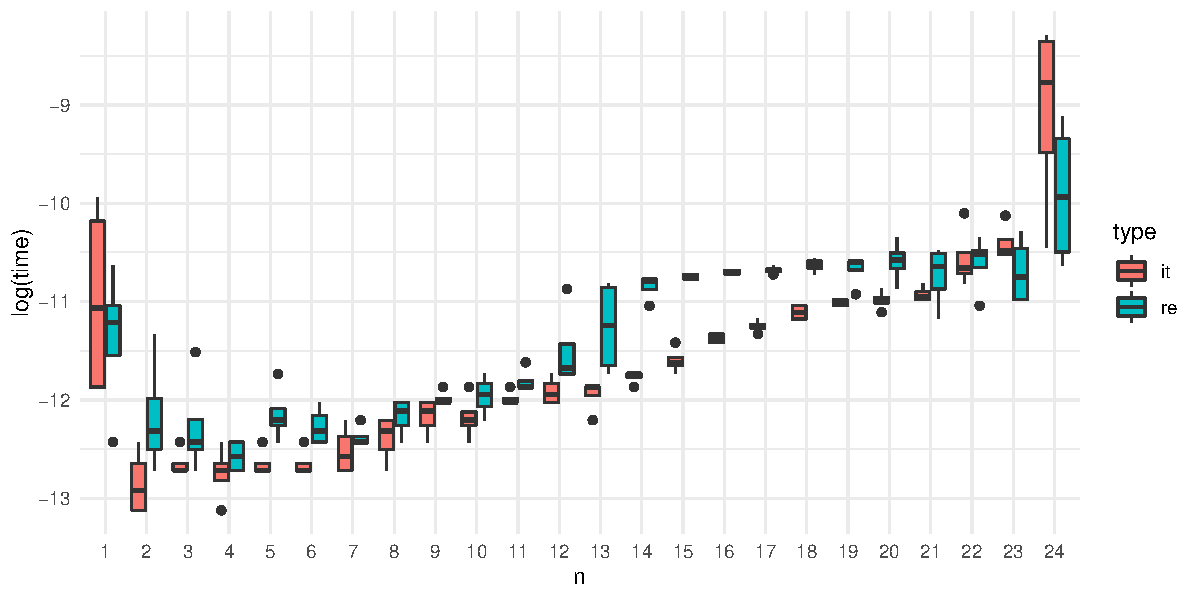
\includegraphics[width=\linewidth]{bs.pdf}
  \caption{Resultados del diseño experimental con $k=5$ ejecuciones para cada tipo de implementación e instancia de prueba de la búsqueda binaria}
  \label{fig:bs}
\end{figure}


Los resultados muestran que existe una mejora menor en el tiempo de ejecución de la implementación recursiva respecto a la iterativa, sin embargo, no es concluyente, ya que al incrementar el tamaño de la instancia esta diferencia se muestra poco clara. Sería necesario realizar un diseño experimental más exhaustivo con un número mayor de repeticiones para lograr un argumento concluyente.
\end{document}
